\chapter{引言}

\section{信息可视化}
信息可视化是一门建立于人类视觉系统感知特性的基础之上,研究图形化数据表征的跨学科研究领域,主要关注于几类特征鲜明的数据类型,包括多维数据、文本、网络与树型数据、时空数据等。它与计算机图形学、人机交互、心理学等相互交叉,也和统计学、机器学习、数据库系统等相辅相成。通过视觉隐喻以及灵活的人机交互,信息可视化将计算机的算力和人的认知结合在一起,能够发挥出与统计模型、自动化数据挖掘算法等截然不同的分析作用。
\draft{有效在什么地方}

随着大数据时代的深入,数据的产生与传播过程均在不断地加速,信息超载和数据过剩等问题带来巨大挑战。一方面,人们需要分析数据,从数据背后隐藏的信息中挖掘出知识和智慧,以此指导实践;另一方面,人们需要通过一些恰当的方式来与外界交流在数据中的认识和发现。而数据可视化正是应对这两种挑战的有力途径。\draft{举例}



\section{文本可视化}

文本是一种典型的非结构化数据,存在于社交媒体、邮件、文档等与人们日常生活息息相关的场景中,是互联网中最主要的结构类型。文本可视化主要关注于待分析语料所蕴含的语义特征,例如词频、主题、情感、逻辑结构、动态演变等,涉及以下三个方面:(1)文本分析——结合自然语言处理的相应技术,提取文本中的信息作为待可视化的特征。(2)可视化呈现——针对特征选择恰当的视觉编码。(3)人机交互——通过一系列的交互切换不同具有内在关联的视图,动态展现数据的不同层面。

\begin{figure}[htbp]
	\centering
	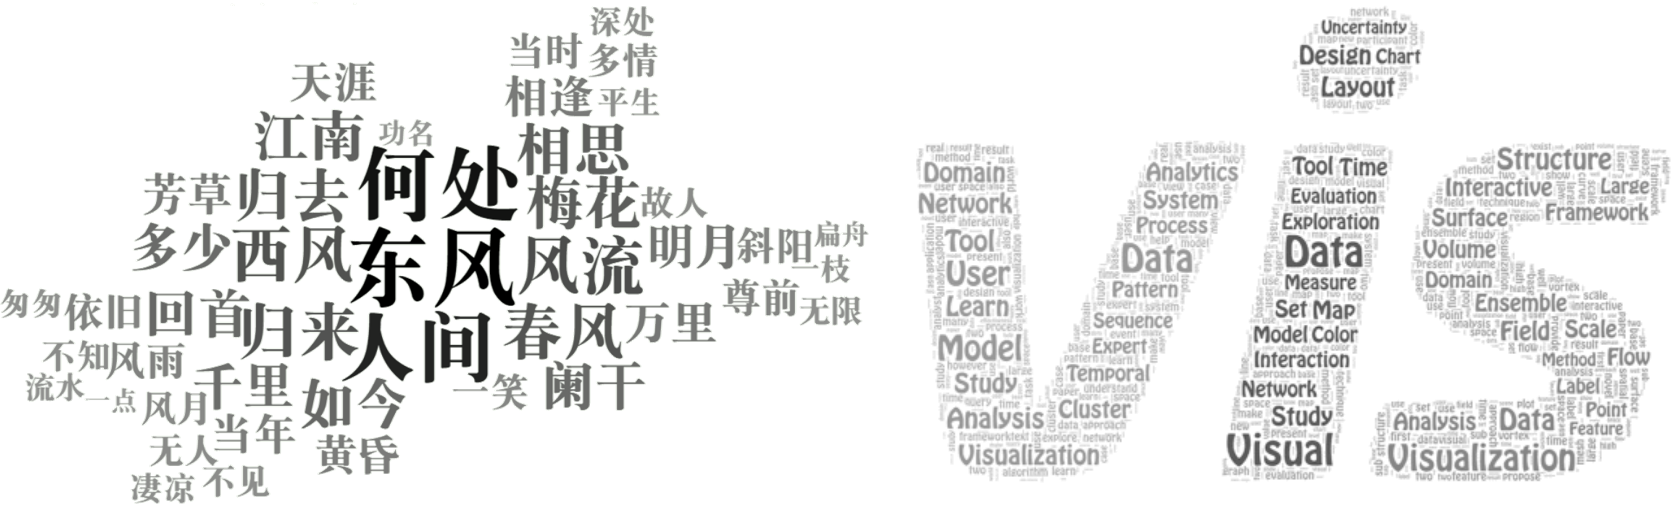
\includegraphics[width=\textwidth]{figures/wordle_example.png}
	\caption{词云示例。左:《全宋词》高频词\protect\footnotemark;右:ShapeWordle~\supercite{Wang2020}。}
	\label{fig:wordle_example}
\end{figure}

\footnotetext{宋词缱绻,何处画人间. \url{http://fms.news.cn/swf/2018_sjxw/quansongci}}

词云是文本可视化中的经典方法,通过字号编码词频,以此呈现文本特征(见图~\ref{fig:wordle_example})。它最早可追溯到1976年Milgram对心理地图的研究~\supercite{milgram1976}。进入Web2.0时代后,它广见于网络博客与论坛,用以展示各标签、主题的热度,并衍生出了歌词概览~\supercite{Burch2016}等丰富的应用。词云的可视化手段还能够有效地概括大型文本数据并支持进一步的探索分析。在往届IEEE VAST可视分析挑战赛中,不乏竞赛团队通过利用词云而挖掘到线索的经典案例\draft{(例子文献)}。


\section{本文工作及创新点}
词云因其色彩丰富而设计感十足的外观与简洁易懂的解读方式被大量地运用于文本分析或展示,成为当今最受欢迎的可视化形式之一。然而,它在提供关键词时并未具体给出该词所对应的语境,无法准确反映文本的主体内容。此外,由于一般的词云布局算法以优化整体紧凑程度为主,词语间的邻近程度与其语义毫无关联,读者难以从中梳理出逻辑,构建对词云的整体理解。

\begin{figure}[htbp]
	\centering
	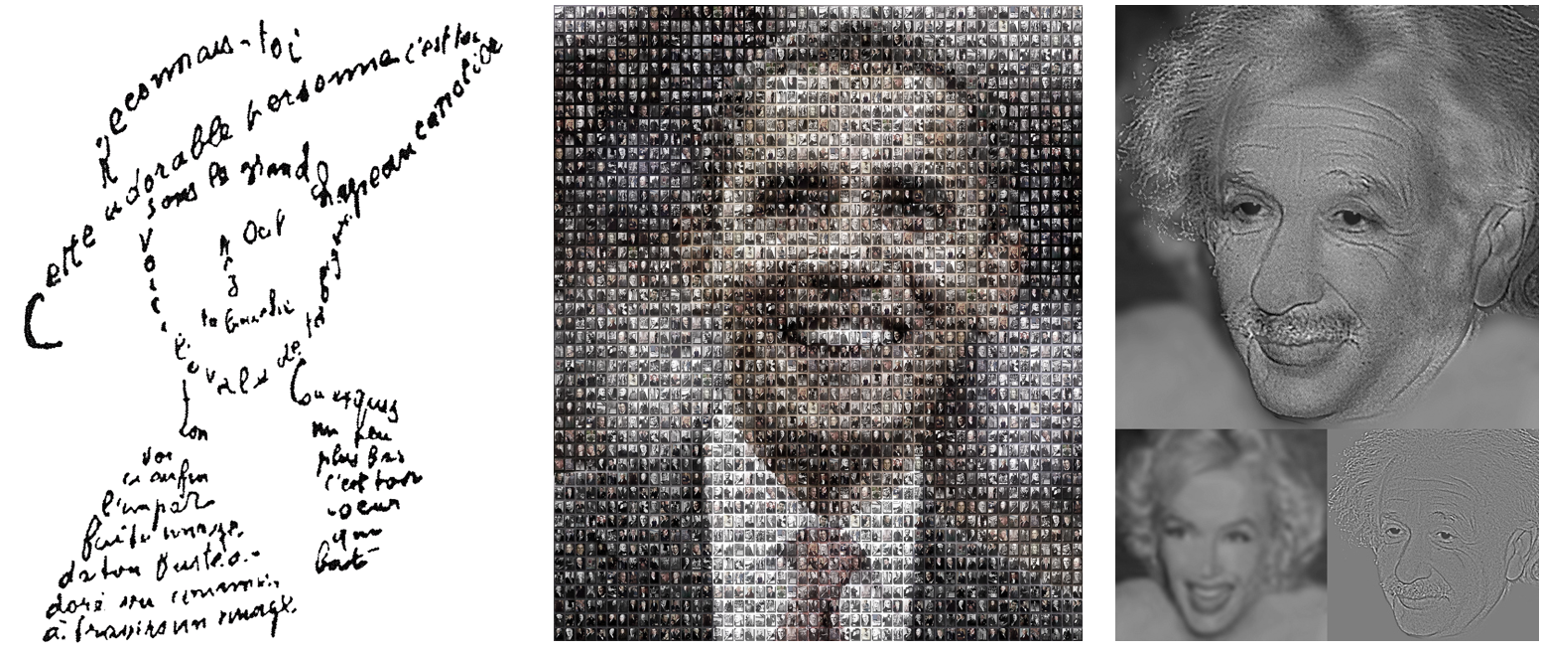
\includegraphics[width=\textwidth]{figures/intro.png}
	\caption{左:图像诗~\supercite{apollinaire1971selected};中:图片马赛克示例;右:混合图像示例~\supercite{Olivia2006}。}
	\label{fig:intro}
\end{figure}


本研究主要是受到多分辨率图像的启发,希望以多分辨率的方式将上下文信息嵌入词云中,在尽可能保留词云美观程度的基础上增加信息的层次,提高词云对文本数据分析的效用,属于一种较为通用的可视化技术。多分辨率图像(示例见图~\ref{fig:intro})在同一图片上用不同编码信息,一般侧重于增强内容的趣味性。例如,法国诗人Guillaume Apollinaire在1915年所开创的图像诗通过精巧的字母布局,将诗句拼凑为相关客体的写意,营造诗与画相谐成趣的效果。又如照片墙常见的的图片马赛克,或者一度引人注目的爱因斯坦与玛丽莲·梦露的混合图像。由于一个关键词往往对应大量的上下文,我们主要考虑在大型显示设备上的双分辨率词云使用场景,以利用其面积大、分辨率高的特性。

本研究的贡献主要包含以下几点:

\begin{itemize}
	\item \textbf{提出了一个新颖的双分辨率词云可视化形式,并设计了相应的生成算法}。这一可视化拓展了词云可视化的设计空间,能够在同一张静态图像上同时编码关键词及上下文信息,弥补现有词云无法提供语境的问题,使分析人员、读者能够更为准确地理解数据,挖掘文本背后的信息。该方法亦可扩展到层次文本数据可视化,具有良好的应用前景。
	
	\item \textbf{基于真实数据构建三个样例,证实了双分辨率词云的有效性}。本研究搜集并整理了《全唐诗》、美国总统特朗普的社交媒体发言以及2020政府工作报告并使用多分辨率词云进行可视化,验证这一方法的有效性。
	
	
	\item \textbf{通过真实案例探究了双分辨率词云的设计空间,实现了一个图形界面以支持用户自定义创制}。对词云布局,目前没有通用的评价准则,且其涉及众多参数,最终结果具有很大的不确定性。为了让用户更好理解参数的意义,我们分析对比了一系列不同参数下的布局结果,并由此给出了一些建议,还提供了一个图形化生成接口支持用户在其他数据上自定义创制双分辨率词云。
	
\end{itemize}

\bigbreak
\bigbreak

\noindent \textbf{文章结构}:本文在第二章介绍相关的感知研究,并对多分辨率技术和词云布局算法进行全面的总结,阐释本研究与现有工作的联系与区别。第三章讨论了多分辨率词云的设计,包括设计目标、设计选择以及早期的实验探索。第四章介绍了本研究提出的双分辨率词云的具体方法。第五章对几个真实数据使用了双分辨率词云可视化,并对其效果进行分析和评价。第六章介绍了协助用户创制双分辨率词云的交互系统。最后,第七章探讨了该研究的应用前景以及未来工作的发展方向。
